\chapter{\MIndex{} implementace v~jazyce Java}


\section{Jazyk Java, JVM}

Jazyk Java je silně typovaný jazyk. Tento jazyk není interpretovaný,
výsledkem překladu je \bytecode{}.\footnote{\bytecode{} jsou instrukce pro JVM. Více viz~\prettyref{sub:JIT}.} Až tento \bytecode{} je interpretován v~tzv. Java Virtual Machine (JVM\nomenclature{JVM}{Java Virtual Machine}).
Díky JVM může kód přeložený na jedné platformě (ať už Windows nebo Unix a 32bit nebo 64bit) běžet na jiné.\footnote{\emph{\uv{Write once, run anywhere}}\cite{lindholm2013java}}

Hlavní klíčové vlastnosti, jak jazyka Java, JVM a JDK\nomenclature{JDK}{Java Development Kit}
jsou tyto: automatická alokace a dealokace paměti, objektovost, generika,
překlad \bytecode{} do nativních instrukcí procesoru, bohatá
knihovna tříd v~základním JDK\ldots{}

\subsection{Automatická správa paměti -- garbage collection\label{sec:memorymanagement}}

V~jazyce Java neexistují ukazatele, pouze reference. V~jazycích C/\CC{}
se musí vývojář starat o~správu paměti pomocí funkcí \method{malloc},
\method{free} (jazyk C a \CC), resp. operátorů \method{new} a \method{delete}
(jazyk \CC). V~jazyce Java, resp. v~JVM \cite{lindholm2013java} tuto starost přebírá tzv. \emph{garbage
collector} (GC\nomenclature{GC}{garbage collector}), který sleduje
dosažitelnost alokovaných objektů v~paměti JVM. Pokud GC
zjistí, že objekt není dosažitelný z~jiných objektů, uvolní pamět daného objektu.
\footnote{Podobná technika/pattern je součástí \CC 11 pomocí \type{std::shared\_ptr},
kde se používá \emph{reference counting} \cite{ISO:2012:CPP}. Tato technika není použitelná v~případě cyklických referencí. Při výskytu cyklických referencí by se měl použít i \type{std::weak\_ptr}.
}

Díky automatické správě paměti je vývoj výrazně rychlejší.
Automatická správa paměti ovšem neznamená, že program je chráněn proti všem únikům paměti.\footnote{V anj. \emph{memory leaks}.}
Pokud se např. \uv{opomene} odstranit záznam z~mapy, odkazovaná instance nikdy nebude uvažována pro GC a vznikne únik paměti.

\subsubsection{Jak funguje GC}
Ve většině JVM se používá generační GC, který vychází ze dvou vypozorovaných chování:
\begin{itemize}
  \item Většina alokovaných objektů je velmi brzy nepotřebná, tzn. nejsou na ně žádná reference
  \item Jen několik starších objektů odkazuje na mladší objekty
\end{itemize}
Tato dvě pozorování jsou známa jako \emph{slabá generační hypotéza}\cite{hunt2011java},\footnote{V anj. \emph{weak generational hypothesis}.} která platí pro většinu programů v~jazyku Java.
K~využití této hypotézy je v~JVM rozdělena \emph{halda}\footnote{V anj. \emph{heap}} na dvě fyzické části, které jsou odkazované jako generace:

\begin{figure}[h]
\centering
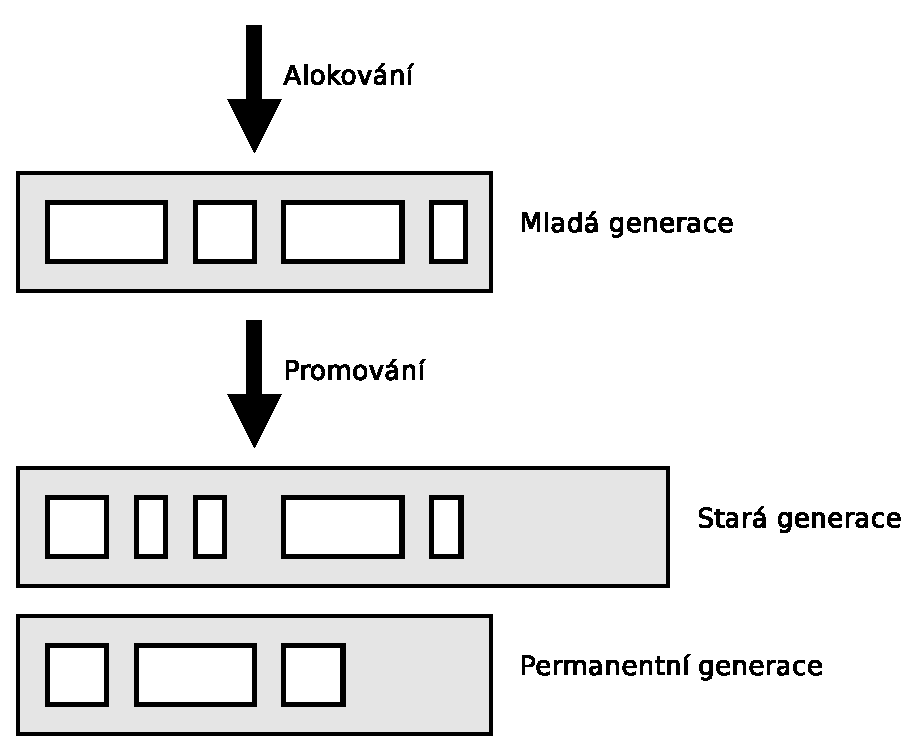
\includegraphics[width=0.5\textwidth]{jvm_memory}
\caption{Rozdělení, alokování a promování paměti v~JVM}
\label{fig:jvm_memory}
\end{figure}

\begin{description}
  \item[Mladá generace] Většina objektů je alokována do této oblasti, která je relativně malá a je často \uv{uklízena}.
Jelikož je předpoklad, že objekty jsou velmi rychle nepotřebné, jen velmi málo objektů \uv{přežije} úklid v~této oblasti.
Obecně je úklid v~této oblasti velmi efektivní, protože je prováděn v~malé oblasti paměti, která obsahuje hodně odpadních objektů.

  \item[Stará generace] Objekty, které \uv{žijí} déle, jsou promovány do této oblasti.
Tato oblast je výrazně větší než \emph{mladá generace} a její obsazování probíhá pomalu.
Úklid v~této oblasti (nazývaný \emph{full GC}) není častý, ale pokud už k~němu dojde, může být velmi dlouhý.

  \item[Permanentní generace] JVM používá tuto třetí generaci pro ukládání metadat, jako jsou informace o~třídách, internovaných řetězců a podobně.
Tato generace není součástí generační hierarchie.

\end{description}

\subsubsection{Typy GC\label{subsub:gctypes}}

V~Oracle JVM je k~dispozici několik GC, lišících se způsobem provádění úklidu a dochází-li k~tzv. \emph{zastavení světa}.\footnote{V anj. \emph{stop the world}}
%%%% jak s tim stop world
\emph{Zastavení světa} znamená, že všechna vlákna programu jsou pozastavena a pouze vlákna pro úklid jsou v~činnosti.
Děje se tak proto, aby nedocházelo k~novým alokacím objektů během úklidu.
Pokud k~zastavení dochází často, má to samozřejmě negativní dopad na aplikaci.

\prettyref{tab:gcs} obsahuje porovnání GC a vyjadřuje, jakým způsobem probíhá úklid paměti jednotlivých generací.

\begin{table}
\center
\begin{tabular}{|l || l | l | p{2cm} | p{2cm} |}
\hline
& Serial GC & Parallel GC & CMS GC & G1 GC \\ \hline \hline
Paralelismus & Ne & Ano & Ano & Ano \\ \hline
Souběžnost & Ne & Ne & Ano & Ano \\ \hline
Úklid mladé gen. & Sériově & Paralelně & Paralelně & Paralelně \\ \hline
Úklid staré gen. & Sériově & Paralelně & Paralelně \& \mbox{Souběžně} & Paralelně \& \mbox{Souběžně} \\
 \hline
\end{tabular}
\caption{Porovnání GC}
\label{tab:gcs}
\end{table}

\subsection{Generika\label{sub:generika}}

Obdobně jako v~\CC{} jsou \emph{templates}\cite{ISO:2012:CPP}, jazyk Java má \emph{generics}.\footnote{Uvedeny ve verzi 1.5 \cite{gosling2013java}.}
Rozdíly jsou následující:
\begin{itemize}
  \item v~Java se informace o~typu ztrácí během překladu. Překladač nahrazuje výskyt generika za konkrétní typ (třída, rozhraní)
  \item nelze jako typový parametr použít primitivní typ -- \type{int, char, byte, long, double, float} \ldots{}
  \item nelze použít netypový parametr
\end{itemize}

Zřejmě největším přínosem je typová bezpečnost při práci s~kolekcemi a možnosti typové specializace.

\subsection{Překlad \bytecode{} do nativních instrukcí procesoru}

JVM je heap procesor.
Kvůli emulaci a virtualizaci procesoru je běh samotného \bytecode{} relativně pomalý.
JVM proto překládá za běhu \bytecode{} do nativních instrukcí procesoru, nad kterým aktuálně JVM běží.
V~JVM od Oracle se tento překladač nazývá JIT\nomenclature{JIT}{Just In Time Compiler}\cite{hunt2011java}.
Samozřejmostí je optimalizace při několika průchodech kódem -- např. \emph{function inlining}, \emph{loop unrolling} nebo \emph{dead code elimination}\cite{hunt2011java}.
Toto jsou velmi důležité vlastnosti, které mohou zásadním způsobem ovlivnit měření výkonnosti programu. Více viz~\prettyref{sec:vykonvjava}.

\subsection{Bohatá knihovna tříd v~základním JDK}

Java je dodávána s~rozsáhlou knihovnou JDK. Obsahuje vše nutné
pro síťovou komunikaci (RPC\nomenclature{RPC}{Remote Procedure Call}), práci s~textem -- regulární výrazy,
XML, soubory a souborový
systém a také velmi propracovanou knihovnou kontejnerů -- \emph{Java
Collections Framework }(JCF\nomenclature{JCF}{Java Collections Framework}). \footnote{V~jazyce Java se používá pro termín \emph{container} (\CC) termín \emph{collection}}

\section{Návrh a implementace}
Implementace \MIndex{u} je napsána pro verzi Java 7.
V~celém návrhu jsem se snažil co nejvíce používat objektově orientovaný přístup.
Tzn. že jsem se maximálně snažil omezit používaní nižších konstrukcí jazyka Java jako jsou pole a spíše využívat knihovny JDK a vyšších konstrukcí jako jsou seznamy, fronty.
Všechny implementované třídy a rozhraní jsou typově parametrizované (viz \prettyref{sub:generika}).

Při některých výpočtech bylo možné použít \emph{rozděl a panuj}\cite{Cormen:2001:IA:580470}\footnote{V anj. \emph{Divide-and-Conquer}} s~využitím \emph{Executor Framework} z~JDK.

V~popisovaných algoritmech (ať už \BPTree{} nebo \MIndex{} je často uváděna proměnná \type{leaf}, resp. zda je daná struktura list -- koncový uzel.
Z~hlediska objektového návrhu se mění chování třídy podle její datové složky, což nesvědčí o~dobrém objektovém návrhu.
K~odstranění toho jsem použil \emph{Replace Type Code with Subclasses}\cite{fowler1999refactoring} pro \BPTree{}.
V~případě \MIndex{} \emph{Range Query} jsem použil \emph{Visitor pattern}\cite{gamma1995design}.

\emph{Visitor pattern} slouží k~oddělení algoritmu od objektové struktury nad kterou se pracuje.
Clustery \MIndex{u} slouží pouze k~udržení informace o~stavbě indexu.
Pokud by se zde použila dědičnost pro odstranění identifikace typů, muselo by se předávat několik objektů do clusteru při jeho konstrukci a také přenést část kódu \emph{Range Query} do implementací \type{Cluster}.
Ve výsledku by tento postup znepřehlednil a zvýšil složitost kódu clusterů.
Použití \emph{Visitor pattern} je elegantní řešení s~jasně rozdělenou zodpovědností mezi třídami.

K ověření funkčnosti jednotlivých částí kódu jsou použity \emph{unit testy} s~pokrytím více jak \SI{70}{\percent}.
Nebyly pokryty jednoduché metody.
Tyto testy zabránily regresím při změnách v~kódu.

\subsection{\BPTree}
Implementace \BPTree{} se nachází v~třídě \linebreak \type{cz.rank.vsfs.btree.BPlusTreeMultiMap}. Tato mapa je typově parametrizována pro klíč a hodnotu. Protože strom musí být setříděný, musí klíč implementovat rozhraní \type{java.lang.Comparable}. Mapa umožňuje ukládat více objektů pod stejným klíčem\footnote{V \CC{} je obdobný kontejner \type{std::multimap}\cite{ISO:2012:CPP}. V~JDK žádná takováto kolekce není.} a umožňuje vyhledání v~intervalu.

Implementace mazání objektů z~mapy není potřebná pro \MIndex{} a není tudíž ani implementována.

Celý \BPTree{} je uložen v~hlavní paměti a není tedy implementováno načítání a ukládání uzlů na disk.

\subsection{\MIndex{}}
Celá implementace \MIndex{} pracuje s~objekty, které implementují rozhraní \type{cz.rank.vsfs.mindex.Distanceable}.
Rozhraní \type{Distanceable} má pouze jednu metodu \method{double distance(Distanceable d)}, která vrací vzdálenost objektu od \method{d}.
Tím je zajištěna případná znovupoužitelnost kódu pro jiné datové typy než je vektor.

\begin{figure}
\centering
\begin{mpost}[use,mpsettings={input metauml;}]

Interface.Distanceable("Distanceable")
	("+distance(object:D):double");
ClassTemplate.TDistanceable("D")(Distanceable);

drawObjects(Distanceable, TDistanceable);
\end{mpost}

\caption{\type{Distanceable} UML diagram}
\end{figure}

\subsubsection{Výpočet maximální vzdálenosti mezi prvky}
Pro výpočet maximální vzdálenosti byla implementována metoda hrubou silou, kdy se počítají vzájemné vzdálenosti všech prvků v~množině a vybere se vzdálenost, která je největší pro dva objekty.
Asymptotická složitost je \BigO{n^2}, protože se množina prochází ve dvou smyčkách.
K~výpočtu lze použít \emph{rozděl a panuj}, takže je celý výpočet paralelní a doba výpočtu se lineárně snižuje s~počtem výpočetních vláken, ale roste kvadraticky s~počtem prvků v~množině.

Funkcionalita je implementována ve třídě \linebreak \type{cz.rank.vsfs.mindex.MaximumDistance}.
Vzdálenost může být spočítána pouze nad objekty, které implementují rozhraní \type{Distanceable}.

\subsubsection{Výpočet vzdáleností mezi pivoty a prvky}
K~výpočtu a seřazení vzdáleností pivotů od objektu slouží třídy implementující rozhraní \type{cz.rank.vsfs.mindex.PivotDistanceTable}. Implementovány jsou tři třídy s~tímto rozhraním:

\begin{figure}
\centering
\begin{mpost}[use,mpsettings={input metauml;}]

Interface.A("PivotDistanceTable")
	("+calculate()",
	 "+pivotAt(object:D, index:int):Pivot<D>",
	 "+firstPivotDistance(object:D):double",
	 "+distanceAt(object:D, index:int):double",
	 "+pivotDistance(object:D, pivotIndex:int):double",
);

ClassTemplate.TA("Distanceable<D>")(A);

AbstractClass.B("AbstractPivotDistanceTable")
	()();
ClassTemplate.TB("Distanceable<D>")(B);
Class.C("ParallelPivotDistanceTable")
	()();
ClassTemplate.TC("Distanceable<D>")(C);

Class.D("SimplePivotDistanceTable")
	()();
ClassTemplate.TD("Distanceable<D>")(D);

Group.g(C,D);

topToBottom.midx(30)(A,B,g);
leftToRight(80)(C,D);

drawObjects(A, B, g, TA, TB, TC, TD);
clink(realization)(B,A);
link(inheritance)(pathStepY(C.n,B.s,10));
link(inheritance)(pathStepY(D.n,B.s,10));

\end{mpost}

\caption{\type{PivotDistanceTable} UML diagram}
\end{figure}

\begin{description}
\item[ParallelPivotDistanceTable] Rozdělí úlohu na menší části podle objektů pomocí \emph{rozděl a panuj} a výpočet je paralelizován za použití všech dostupných jader systému. Tato třída je využita při konstrukci samotného \MIndex{}.
\item[SimplePivotDistanceTable] Podobně jako \type{ParallelPivotDistanceTable} vypočte vzdálenosti objektu od pivotů, ale pouze pro jeden objekt a výpočet není paralelní. Tato třída se používá v~samotném \emph{Range Query} dotazu. Pokud by se použil \type{ParallelPivotDistanceTable}, tak čas spojený s~vytvářením úloh pro exekutory a vytvářením vláken, by byl výrazně vyšší než samotný výpočet vzdáleností jednoho objektu.
\item[AbstractPivotDistanceTable] Je společným předkem obou výše uvedených tříd a obsahuje společný kód, který potomci využívají.
\end{description}

\subsubsection{Cluster tree}
\begin{figure}
\centering
\begin{mpost}[use,mpsettings={input metauml;}]

Interface.ClusterVisitor("ClusterVisitor")
	("+enterInternalCluster(internalCluster:InternalCluster<D>)",
	 "+enterLeafCluster(leafCluste:rLeafCluster<D>)");
ClassTemplate.TClusterVisitor("Distanceable<D>")(ClusterVisitor);

Interface.Cluster("Cluster")
	("+getIndex():Index",
	 "+accept(visitor:ClusterVisitor<D>)",
	 "+getLevel():int",
	 "+getSubCluster(pivot:Pivot<D>):Cluster<D>",
);

ClassTemplate.TCluster("Distanceable<D>")(Cluster);

Note.InternalClusterCode("visitor.enterInternalCluster(this)");
Class.InternalCluster("InternalCluster")
	()("+accept(visitor:ClusterVisitor<D>)",);
InternalClusterCode.nw = InternalCluster.se - (5, 10);
ClassTemplate.TInternalCluster("Distanceable<D>")(InternalCluster);

Note.RootClusterCode("foreach subcluster do:"," subcluster.accept(visitor)");
Class.RootCluster("RootCluster")
	()("+accept(visitor:ClusterVisitor<D>)",);
RootClusterCode.nw = RootCluster.sw - (0, 10);
ClassTemplate.TRootCluster("Distanceable<D>")(RootCluster);

Note.LeafClusterCode("visitor.enterLeafCluster(this)");
Class.LeafCluster("LeafCluster")
	()("+accept(visitor:ClusterVisitor<D>)",);
LeafClusterCode.nw = LeafCluster.sw - (0, 10);
ClassTemplate.TLeafCluster("Distanceable<D>")(LeafCluster);

Group.g(RootCluster,LeafCluster);

topToBottom.midx(40)(ClusterVisitor, Cluster,InternalCluster,g);
leftToRight(50)(RootCluster,LeafCluster);

drawObjects(ClusterVisitor, Cluster, InternalCluster, g, TClusterVisitor, TCluster, TInternalCluster, TRootCluster, TLeafCluster, InternalClusterCode, RootClusterCode, LeafClusterCode);
clink(realization)(InternalCluster,Cluster);
link(inheritance)(pathStepY(RootCluster.n,InternalCluster.s,10));
link(inheritance)(pathStepY(LeafCluster.n,InternalCluster.s,10));

clink(dashedLink)(InternalCluster.methodStack.pict[0], InternalClusterCode);
clink(dashedLink)(RootCluster.methodStack.pict[0], RootClusterCode);
clink(dashedLink)(LeafCluster.methodStack.pict[0], LeafClusterCode);
\end{mpost}

\caption{\type{Cluster} UML diagram s \emph{Visitor pattern}}
\end{figure}

Cluster tree je tvořen třídami, které implementují rozhraní \linebreak \type{cz.rank.vsfs.mindex.Cluster}. Jsou celkem 3 -- 
\type{InternalCluster} a jeho potomci  \type{LeafCluster} a \type{RootCluster}.

\begin{description}
\item[InternalCluster] Je použit jako vnitřní cluster. Obsahuje všechnu funkcionalitu pro udržení informací o~podstromech, objektech, informace o~minimální a maximální vzdálenosti uložené v~clusteru.
\item[LeafCluster] Reprezentuje koncový cluster. Jeho metoda \linebreak \method{LeafCluster.getSubCluster} vrací vždy konstantu \type{NO\_SUBCLUSTERS}. Toto slouží k~identifikaci koncového clusteru při utváření dynamického \MIndex{u}.
\item[RootCluster] Je použit pro kořen celého clusteru, protože vyžaduje speciální zacházení s~indexem a také při akceptování \type{ClusterVisitor}.
\end{description}

Pro změření rozdílu použití více-stupňového \MIndex{u} a \MIndex{u} s~dynamickými stupni jsou implementovány dvě třídy -- \linebreak \type{cz.rank.vsfs.mindex.MultiLevelClusterTreeBuilder} a \linebreak \type{cz.rank.vsfs.mindex.DynamicClusterTreeBuilder}. Tyto třídy jsou použity v~\type{cz.rank.vsfs.mindex.MultiLevelMIndex}, \linebreak resp. \type{cz.rank.vsfs.mindex.DynamicMIndex} ke konstrukci specifického \MIndex{u}.
Obě třídy mají téměř totožný konstruktor, pouze \linebreak u~\type{DynamicClusterTreeBuilder} je navíc parametr pro maximální zaplnění koncového clusteru. Více viz \prettyref{sec:Dynamic-Cluster-Tree}.

\subsubsection{Range Query}
Díky nezávislosti dotazu na typu clusteru (vícestupňový vs. s~dynamickými stupni) je \emph{Range Query} implementován v~třídě \type{MIndex}, která je společným rodičem pro \type{MultiLevelMIndex} a \type{DynamicMIndex}.
V~metodě \method{MIndex.rangeQuery} není celá logika vyhledávání.
 V~této metodě se inicializuje \type{ClusterRangeQuery}, která implementuje rozhraní \type{ClusterVisitor} a také samotné vyhledávání.
Toto řešení jsem zvolil kvůli oddělení zodpovědnosti vyhledávání a uchovávání informací o~\MIndex{u}.\footnote{Jedná se o~tzv. \emph{Single Responsibility Principle\nomenclature{SRO}{Single Responsibility Principle}}\cite{martin2003agile}}

V~podstatě je téměř doslovně přepsán algoritmus popsaný v~\prettyref{sec:Range-Query}.
Jak bylo již zmíněno v~začátku této sekce, k~odstranění nutnosti identifikování typu clusteru za běhu\footnote{V jazyce Java k~identifikaci typu slouží operátor \method{instanceof}\cite{gosling2013java}, obdobně jako v~\CC{} je operátor \method{typeid}\cite{ISO:2012:CPP}} je použit \emph{Visitor Pattern}. \prettyref{fig:rangequery-visitor-seq} popisuje toto volání detailně.

\begin{figure}[p]
\footnotesize
%\begin{sideways}
\begin{sequencediagram}
  \newthread{mi}{:MIndex}{MIndex}
  \newinst[1]{crq}{crq:ClusterRangeQuery}
  \newinst[2]{cq}{cq:Queue<Cluster<D{>}>}
%  \newinst{ic}{:InternalCluster}
%  \newinst{lc}{:LeafCluster}
%  \sidelabel{mi}{left}{rangeQuery(D, range)}

  \begin{call}{mi}{performQuery()}{crq}{nalezené objekty}
       \begin{call}{crq}{addAll(root.getSubclusters())}{cq}{}
       \end{call}
     \begin{sdblock}{loop}{cq není prázdná}
       \begin{call}{crq}{poll()}{cq}{cluster}
       \end{call}
       \begin{sdblock}{opt}{[!doublePivotDistanceConstraint(...)]} 
         \begin{sdblock}{alt}{[InternalCluster]}
        \begin{sdblock}{ref}{sd InternalCluster}
         \separateline{crq}{crq}
        \end{sdblock}
         \separateline{crq}{cq}
           \begin{altblock}{crq}{LeafCluster}{cq}
         \begin{sdblock}{ref}{sd LeafCluster}
         \separateline{crq}{crq}
          \end{sdblock}
         \end{altblock}
       \end{sdblock}	
     \end{sdblock}	
   \end{sdblock}
 \end{call}
\end{sequencediagram}
%\end{sideways}

\caption{Sekvenční diagram volání \emph{Range Query}}
\label{fig:rangequery-visitor-seq}
\end{figure}

\begin{figure}[ht]
\footnotesize
\begin{sequencediagram}
  \newthread{crq}{crq:ClusterRangeQuery}
  \newinst[2]{cq}{cq:Queue<Cluster<D{>}>}
  \newinst{ic}{ic:InternalCluster}
% \sidecall{mi}{left}{rangeQuery(D, range)}

\begin{sdblock}{sd}{InternalCluster}
       \begin{call}{crq}{accept(this)}{ic}{}
           \begin{call}{ic}{enterInternalCluster(this)}{crq}{}
           \begin{call}{crq}{addAll(ic.getSubClusters())}{cq}{}
           \end{call}
           \end{call}           
       \end{call}
\end{sdblock}
\end{sequencediagram}

\caption{Sekvenční diagram volání \emph{Range Query} pro \type{InternalCluster}}
\label{fig:rangequery-visitor-seq-internal}
\end{figure}

\begin{figure}[ht]
\footnotesize
\begin{sequencediagram}
  \newthread{crq}{crq:ClusterRangeQuery}
  \newinst[2]{bt}{bt:BPusTreeMultiMap}
  \newinst{fo}{fo:List<D>}
%  \newinst{ic}{:InternalCluster}
  \newinst{lc}{:LeafCluster}
%  \sidelabel{mi}{left}{rangeQuery(D, range)}

\begin{sdblock}{sd}{LeafCluster}
       \begin{call}{crq}{accept(this)}{lc}{}           
           \begin{call}{lc}{enterLeafCluster(this)}{crq}{}
           \begin{sdblock}{opt}{[!rangePivotDistanceConstraint(...)]}
              \begin{callself}{crq}{rangeSearchForObjects(keyMin)}{objects}
                 \begin{call}{crq}{rangeSearch(r1, r2)}{bt}{objects}
                 \end{call}
              \end{callself}
           \begin{sdblock}{loop}{objects}
           \begin{sdblock}{opt}{[!pivotShouldBeFiltered(object, ...)]}
           \begin{sdblock}{opt}{[!isObjectInRange(object, ...)]}
                 \begin{call}{crq}{add(object)}{fo}{}
                 \end{call}
           \end{sdblock}
           \end{sdblock}
           \end{sdblock}
           \end{sdblock}
           \end{call}
       \end{call}           
\end{sdblock}
\end{sequencediagram}

\caption{Sekvenční diagram volání \emph{Range Query} pro \type{LeafCluster}}
\label{fig:rangequery-visitor-seq-leaf}
\end{figure}

\section{Měření výkonu v~Java\label{sec:vykonvjava}}

Abychom porozuměli úskalí měření výkonu kódu v~JVM, je nejprve nutné si přiblížit, co se děje uvnitř JVM, jak probíhá překlad a optimalizace kódu.

\subsection{Zavádění tříd}

Všechny třídy jsou přeloženy do \classfile{} souborů. Ty mohou být následně zabaleny do JAR\nomenclature{JAR}{Java ARchive}, což je v~podstatě ZIP archív. JVM při startu vyhledá tzv. Main-Class a k~ní všechny závislé třídy a k~nim další závislé třídy v~tzv. \emph{classpath}. U~každé třídy se provede statická inicializace. Toto vyhledávání není omezeno pouze na úvodní spuštění JVM. Volání \method{Class.forName()}, \method{ClassLoader.loadClass()}, \emph{Reflection API} a \method{JNI\_FindClass} může vyvolat \emph{zavádění tříd}\footnote{V anj. \emph{class loading}} kdykoliv za běhu programu, pokud požadovaná třída není již nahrána\cite{gosling2013java}\cite{lindholm2013java}.

Další fází při \emph{zavádění tříd} je i verifikace \bytecode{}. Všechny překladače Java (\javac{}) vytvářejí validní \classfile{} soubory a typově bezpečný kód. Jenže JVM se nemůže spolehnout, že soubor, který nahrála je správný. Proto musí ověřit, že je vše v~pořádku -- ať již instrukce zadané v~\classfile{} souboru nebo typová bezpečnost.

Výše popsaný proces \emph{zavádění tříd} je velmi náročný na I/O operace a zásadním způsobem ovlivní výsledek měření, pokud se nepředejde tomuto zavádění během měření.

\subsection{JIT\label{sub:JIT}}
Tradiční překladače (např. C/\CC) generují z~vyššího programovacího jazyka strojově závislý kód. Tento kód má finální podobu a všechny možné optimalizace je zapotřebí udělat během překladu. Případně použít profilování výsledné binárky a znovu nechat překladač znovu přeložit kód s~využitím profilovacích dat. Těmto překladačům se říká také statické. Výsledný kód je optimalizován pro danou platformu.

Java používá překladač \javac{}, který z~vysokoúrovňového jazyka vytvoří \classfile{} soubor, obsahující \bytecode{}. JVM tento \bytecode{} následně dynamicky za běhu překládá do strojově závislého kódu pomocí JIT.

\subsubsection{Jak funguje překladač}
Každý překladač má podobnou strukturu.
Musí mít na vstupu modul pro převod zdrojového kódu do tzv. \emph{intermediate representation (IR)}\nomenclature{IR}{Intermediate Representation}.
IR je reprezentace programovacího jazyka do vnitřní formy překladače.
Existují různé typy IR. Pro každou fázi překladu se dokonce může použít jiný IR.
Všechny překladače dělají největší optimalizace právě na IR.
Množina možných optimalizací může být velmi široká a je často omezena množstvím času nutném k~provedení dané optimalizace.
Mezi jednoduché optimalizace patří zjednodušování logických výrazů, nahrazování proměnných konstantami a \emph{function inlining}.
Složitější optimalizace jsou většinou spojeny se smyčkami -- \emph{loop unrolling}, odstraňování kontroly rozsahu smyčky atd\ldots{}

Když jsou tyto optimalizace hotovy, další modul vezme danou IR a převede ji do strojové podoby. Zde nastávají další optimalizace v~podobě přiřazování hodnot do registrů procesoru, výběr vhodných instrukcí atd\ldots{}

\subsubsection{Kdy JIT překládá do strojového kódu\label{subsub:whenJIT}}
JIT nepřekládá každou instrukci v~\bytecode{} ihned do strojového kódu. Většina instrukcí je na začátku interpretována. Až v~okamžiku, kdy daná instrukce se stane \emph{hot}, JIT ji zařadí pro překlad. JVM totiž udržuje u~každé metody čítač volání. Pokud daná metoda je volána vícekrát, stane se \emph{hot} a tím se vyvolá i její překlad. Hranice překladu je ve výchozím nastavení \num{10000}.\footnote{Parametr pro Oracle JVM, který ovlivňuje toto nastavení je \cmd{-XX:CompileThreshold=}} Zjednodušeně řečeno: aby došlo k~překladu libovolné metody do strojového kódu, musí být daná metoda volána aspoň $\num{10000}\times$.

Níže jsou uvedeny optimalizace, které ovlivňují výkonnost kódu.

\begin{description}
\item[function inlining] Je technika vnořování těla kódu funkcí/metod do těla volané metody. Protože každá metoda třídy je v~jazyce Java virtuální, tato optimalizace odstraňuje penalizaci za jejich volání. Ve výsledku vytváří velké bloky kódu, nad kterými se uplatňují další optimalizace. K~vnořování nedochází u~všech metod. Podmínkou je, aby metoda byla krátká, což znamená, aby měla velikost do 35 \bytecode s.\footnote{V Oracle JVM lze toto omezení upravit pomocí parametru \cmd{-XX:FreqInlineSize=}} Vnořování nemůže být vynuceno. Záleží na JIT. Není ani žádné doporučení pro kompilátor jako je tomu u~\CC{} pomocí vyhrazeného slova \method{inline} u~metody.\footnote{\method{inline} říká kompilátoru, že by mohl metodu vnořit, ale záleží na chytrosti kompilátoru, zda vnoření provede\cite{Stroustrup:1997:CPL:523265}.}

Tato technika má zásadní dopad na běh programu. Ve výsledku nutí programátora navrhnout třídy tak, aby byly tvořeny malými metodami, což má za následek i dobrou čitelnost kódu.

\item[dead code elimination] JIT je schopen při analýze běhu programu identifikovat části kódu, které nemají žádný vedlejší efekt, např. pokud se výsledek volání metody nepoužije v~dalších krocích.
Pokud je měřící kód nesprávně navrhnut, může dojít k~tomu, že díky této optimalizaci se některé části nevykonají a výsledky měření jsou nepoužitelné.

\item[loop unrolling] Slouží k~rozbalení smyček jako je \method{for (...) ...}.
Klasická optimalizace, která tělo smyčky \uv{zkopíruje} několikrát za sebou. Každá smyčka má inkrementální část a podmínku pro ukončení smyčky.
Podmínka pro ukončení má vliv na \emph{předpovídání větvení}\footnote{V anj. \emph{branch prediction}} v~CPU.\footnote{Moderní CPU mají velmi sofistikované algoritmy na předpovídání větvení programu s~předčítáním instrukcí do \emph{pipeline}.
Pokud CPU špatně odhadne následující větev kódu, v~drtivé většině případů musí \uv{zahodit} a znovu načíst instrukce do \emph{pipeline}.
Tato operace je velmi drahá a zastaví na několik cyklů vykonávání instrukcí CPU.}
Ve výsledku se daná podmínka nevyhodnocuje tak často.

\begin{figure}
\begin{lstlisting}[frame=single,language=Java,caption=Před loop unrolling]
for (int x = 0; x < 50; x++) {
  doSomethingWith(x);
}
\end{lstlisting}
\begin{lstlisting}[frame=single,language=Java,caption=Po loop unrolling]
for (int x = 0; x < 50; x+=5) {
  doSomethingWith(x);
  doSomethingWith(x+1);
  doSomethingWith(x+2);
  doSomethingWith(x+3);
  doSomethingWith(x+4);
}
\end{lstlisting}
\end{figure}
\end{description}

\subsection{Zahřátí JVM}

Pokud bychom začali měřit jednotlivé části kódu ihned po startu JVM, neměřili bychom výkonnost samotného kódu, ale i čas za jak dlouho JVM zavede jednotlivé \classfile soubory, za jak dlouho JIT přeloží a optimalizuje instrukce \bytecode{} do strojového kódu.
Pravděpodobně by se i naměřené hodnoty pro stejné testované parametry lišily, protože by k~překladu docházelo v~průběhu nebo mezi jednotlivými měřeními.
Proto je nutno provést tzv. \emph{zahřátí JVM}.\footnote{V anj. \emph{JVM warm-up}}

Zahřátí se provádí tak, že se zavolá měřený kód tolikrát, aby se stal \emph{hot}.\footnote{Viz \prettyref{subsub:whenJIT}}
Po tomto zahřátí, by již měl být měřený kód optimalizován a převeden do strojového kódu a měření by nemělo být ovlivněno.

\subsection{GC během měření}
Jak bylo uvedeno v~\prettyref{subsub:gctypes}, během úklidu paměti může dojít k~zastavení aplikace.
Je otázka, jak k~tomuto zastavení přistupovat při měření.
V~reálné aplikaci je toto běžné a záleží na typu aplikace, zda je zastavení aplikace na určitý časový okamžik problémem nebo ho lze tolerovat.
Podle typu aplikace je tedy vhodné vybrat i správný \emph{garbage collector}.

V~případě testování výkonnosti určitého algoritmu je zřejmě vhodné zabránit úklidu během měření, protože ve výsledném měření bude započítán i čas nutný pro úklid paměti.
Z~aplikace je možné vynutit úklid pomocí voláni \method{System.gc()} a \uv{počkat}, dokud neproběhne úklid paměti.
V~měřeních jsem tohoto volání využil, aby se opravdu měřil čas nutný k~vykonání \emph{Range Query}.

\section{Metoda a výsledky měření}
V~měření implementace \MIndex{u} jsem se zaměřil více na praktičnost a detaily ohledně jazyka Java než na zkoumání ořezávání clusterů samotným \MIndex{em}.
Je to z~toho důvodu, že dle mého názoru původní autoři již popsali a prozkoumali principy ořezávání a jiné techniky v~rámci odborného popisu \MIndex{u}.
 
\subsection{Metoda měření\label{sec:measurementmethod}}

\MIndex{} má několik parametrů, které ovlivňují jeho chování, resp. výkonnost, v~závislosti na velikosti a typu indexovaných dat.
Parametry pro měření jsou následující:
\begin{description}
\item[počet pivotů] (z~kolika pivotů má být vytvořen \MIndex{})
\item[počet vyhl. objektů] (kolik se má vyhledat objektů v~rámci jednoho měření)
\item[max. úroveň clusteru] (platí pro oba dva typy clusterů)
\item[počet měření] (kolik měření se má provést s~danými parametry)
\item[max. počet objektů v~listech] (tento parametr je pouze při měřeních dynamického clusteru a určuje maximum objektů v~listu clusteru)
\item[vzdálenost] (maximální vzdálenost hledaných objektů od vzorového)
\item[stupeň \BPTree{}] (určuje počet klíčů v~uzlech \BPTree{}. Jelikož není implementováno načítání a ukládání uzlů na disk, tento parametr ovlivňuje samotné vyhledávání ve stromu)
\end{description}

Výkonnost \MIndex{u} ovlivňuje i nastavení parametrů JVM.
Zde jsem se rozhodl prozkoumat 2 parametry -- \cmd{-XX:+AggressiveOpts} a \cmd{-XX:+UseCompressedOops}, tzn. jejich vliv na výsledné měření a na jejich kombinace.

\begin{description}
\item[AggressiveOpts] Tato volba povoluje agresivní optimalizace JIT.
Volba je označena jako experimentální a rozsah optimalizací může být jiný v~každé verzi JVM.
\item[UseCompressedOops] Tato volba je dostupná pouze pro 64bitovou verzi JVM a je ve výchozím stavu zapnuta, pokud není vynuceno její vypnutí při startu JVM.
V~JVM jsou všechny ukazatele na objekty shodné se strojovými ukazateli, tzn. na 64bitové architektuře jsou 64bitové, na 32bitové architektuře jsou 32bitové.
Obecně je používání 64bitových instrukcí pomalejší oproti ekvivalentním 32bitovým instrukcím -- pro práci vyžadují totiž i odpovídající registry atd\ldots{}
Při zapnuté volbě \emph{UseCompressedOops} JVM komprimuje ukazatele na 32 bitů a umožňuje používat 64 bitové registry pro jiné operace, čímž snižuje penalizaci za 64 bitové instrukce.\footnote{Toto je velmi jednoduché přiblížení. Více viz \cite{hunt2011java}}
\end{description}


Průběh testu je následující:

\begin{enumerate}
\item Vygenerování parametrů pro měření.
\item Načtení vstupních dat ze souboru a vytvoření vektorů.
\item Výpočet maximální vzdálenosti mezi objekty mimo třídy \type{*MIndex}, aby se pro každé nové měření nemusela znovu počítat vzdálenost.
Každá třída \type{cz.rank.vsfs.mindex.MultiLevelMIndex} a \linebreak \type{cz.rank.vsfs.mindex.DynamicMIndex} má konstruktor, který má parametr pro předpočítanou maximální vzdálenost.
\item Zahřátí JVM.
\item Opakující se test:
\begin{enumerate}
\item Vytvoření pivotů.
\item Vytvoření instance \type{\MIndex{}}.
\item Přiřazení vektorů do instance \type{\MIndex{}}.
\item Vytvoření vnitřní struktury \MIndex{u} voláním metody \method{MIndex.build()}.
\item Spuštění časovače.
\item Jednotlivé dotazy na podobnost voláním \method{MIndex.rangeQuery()}
\item Vypnutí časovače.
\item Vypsání informací o~měření -- parametry a čas vyhledávání
\item Spuštění úklidu paměti.
\end{enumerate}

Výsledné časy byly zprůměrovány.
Časovač zaznamená čas zapnutí a čas vypnutí pomocí \method{System.currentTimeInMillis()} a rozdíl je čas měření v~milisekundách.
Při tomto způsobu se nezaznamenává pouze čas vlákna, kolik taktů bylo aktivní, ale celková doba mezi zapnutím a vypnutím stopek.
Pokud je systém vytížen a měřené aplikaci se nedostává času procesoru, je měření tímto postiženo.
Měření probíhalo v~textovém režimu bez grafického prostředí, aby žádné další uživatelské procesy neovlivňovaly měření.

\end{enumerate}
\subsection{Prostředí}
Měření probíhalo v~tomto prostředí(\prettyref{tab:environment}):

\begin{table}[h]
\catcode`\-=12
\center
\begin{tabular}{|l  | l | c |}
\hline
\multirow{9}{*}{CPU} & \multicolumn{2}{|c|}{AMD Phenom\texttrademark II X4 905e Processor} \\ \cline{2-3}
& Architektura & 64bit \\ \cline{2-3}
& Počet jader & 4 \\ \cline{2-3}
& Počet vláken & 4 \\ \cline{2-3}
& Frekvence & \SI{2,5}{\GHz} \\ \cline{2-3}
&  \multirow{2}{*}{L1 cache} & 4 x 64KB pro instrukce \\
& & 4 x 64KB pro data \\ \cline{2-3}
& L2 cache & 4 x 512 \\ \cline{2-3}
& L3 cache & 6MB \\ \cline{2-3}
\hline
\multirow{3}{*}{RAM} & Velikost & 12GB \\ \cline{2-3}
& Typ & DDR3 \\ \cline{2-3}
& Frekvence & \SI{1333}{\MHz} \\ \cline{2-3}
\hline
\multirow{2}{*}{Operační systém} &  \multicolumn{2}{|c|}{Debian/GNU Linux 7.0}  \\
&  \multicolumn{2}{|c|}{\tiny 3.8-trunk-amd64 \#1 SMP Debian 3.8.3-1~experimental.1 x86\_64 GNU/Linux} \\ \cline{2-3}
\hline
\multirow{2}{*}{Java} & JDK & {\tiny Java(TM) SE Runtime Environment (build 1.7.0\_13-b20)} \\ \cline{2-3}
& JVM & {\tiny Java HotSpot(TM) 64-Bit Server VM (build 23.7-b01, mixed mode)} \\ \cline{2-3}
 \hline
\end{tabular}
\caption{Informace o~prostředí\label{tab:environment}}
\end{table}

\subsection{Parametry měření}
\begin{table}[h]
\center
\begin{tabular}{|l|c|}
\hline
Parametr & Hodnot(a/y) \\ \hline
\hline
počet pivotů & \numlist{10; 20; 30; 50} \\ \hline
počet vyhl. objektů & \num{100} \\ \hline
max. úroveň clusteru & \numlist{2; 3; 4} \\ \hline
počet měření & \num{20} \\ \hline
max. počet objektů v~listech & \numlist{10; 20; 50; 100; 200; 300; 500} \\ \hline
vzdálenost & \numlist{0.15} \\ \hline
řád \BPTree{} & \numlist{50; 100; 500} \\ \hline
počet objektů pro porovnání & \num{68040} \\ \hline
dimenze objektů & \num{32} \\ \hline
\end{tabular}
\end{table}

Původním záměrem bylo změřit více hodnot, např. počet pivotů \num{100} s~max. počtem objektů v~listech \num{10} a úrovní clusteru \num{5}.
Při těchto parametrech byl ovšem počet clusterů extrémně velký -- $100 \times 99 \times 98 \times 97 \times 96 = \num{9034502400}$, a docházelo k~přetečení typu \type{Integer} v~kolekcích a k~nesmyslným výsledkům.\footnote{V~Java je typ \type{Integer} 4 bajtový celočíselný typ se znaménkem a může mít maximálně hodnotu $2^{31}-1$}

Při tomto množství je celkový počet kombinací parametrů \num{252} pro dynamický cluster a \num{36} pro vícestupňový cluster.
Jelikož počet měření je \num{20} pro každý parametr, bylo celkově vykonáno \num{5760} měření.

Každá série měření byla spouštěna s~JVM s~různými kombinacemi parametrů, které byly uvedeny v~\prettyref{sec:measurementmethod}.
Implementace GC byla použita G1.
Pro další výklad jsem se rozhodl použít následující označení:

\begin{table}[h]
\center
\begin{tabular}{|l  || c | c |}
\hline
& AggresiveOpts & CompressedOops \\ \hline
\hline
JVM1 & Zapnuto & Zapnuto \\ \hline
JVM2 & Vypnuto & Zapnuto \\ \hline
JVM3 & Zapnuto & Vypnuto \\ \hline
JVM4 & Vypnuto & Vypnuto \\ \hline
\end{tabular}
\caption{Označení kombinací parametrů JVM}
\end{table}

\subsection{Výsledky měření}
Nejlepšího výsledku, tzn.~v~nejkratším čase, bylo dosaženo s~dynamickým \MIndex{em} s~následujícími parametry: počet pivotů \num{10}, maximální úrovní clusteru \num{4}, maximálním počtem objektů v~listech \num{10} a stupněm \BPTree{} \num{500}.
Výsledný čas byl \SI{3485}{\ms} pro parametry JVM1.
Tato konfigurace dosáhla nejkratšího času i s~ostatními parametry JVM, pouze pro JVM2 byla až \uv{druhá}.
Rozdíl časů mezi maximálně optimalizovaným JVM a nejméně (JVM1 vs JVM4) s~těmito parametry byl více jak \SI{200}{\ms}.

Nejdelší zpracování dotazů bylo u~vícestupňového \MIndex{u} pro JVM4 s~parametry: počet pivotů \num{50}, maximální úrovní clusteru \num{4} a stupněm \BPTree{} \num{10}.
Výsledný čas je \SI{5201}{\ms} a rozdíl oproti nejkratší konfiguraci je více jak \SI{1700}{\ms}.

\prettyref{fig:jvm1p50} zobrazuje nejrychlejší vyhledání v~závislosti na stupni \BPTree{}.
Jsou zobrazeny časy pro jednotlivé nejlepší parametry \MIndex{ů} z~jednotlivých nastavení JVM.
Pro zobrazení zásadního vlivu nastavení JVM je i zobrazen vícestupňový \MIndex{} pro \num{50} pivotů a stupeň clusteru \num{4}.

\begin{figure}[t]
\centering
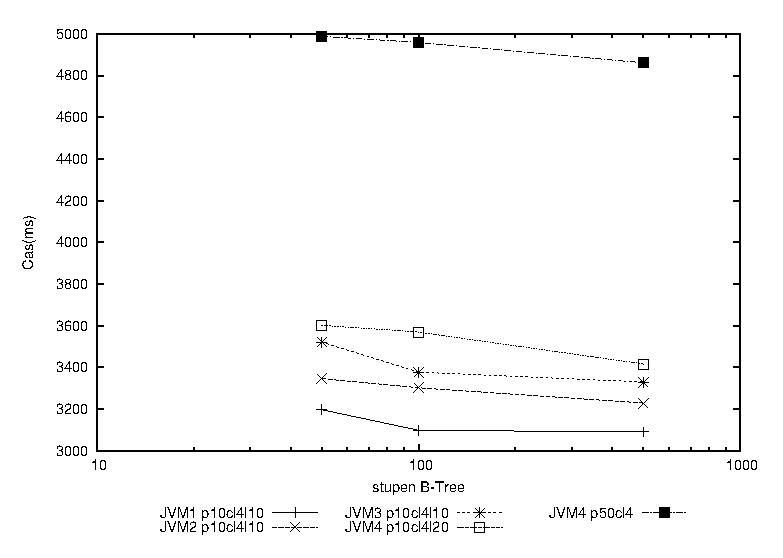
\includegraphics{best_compare}
\caption{Porovnání nejlepších a nejhorších výsledků \emph{Range Query}}
\label{fig:jvm1p50}
\end{figure}

Z~výsledků měření vyplývá, že parametry JVM zásadním způsobem ovlivňují výslednou efektivitu kódu.
\prettyref{tab:jvmavgtime} zobrazuje průměrnou dobu jednoho měření.\footnote{Hodnoty jsou spíše orientační pro posouzení vlivu parametrů JVM.}
Volba \cmd{-XX:+UseCompressedOops} je zásadní pro běh JVM v~64 bitovém prostředí.
Rozhodně není doporučeno tuto volbu vypínat.
Jak bylo uvedeno v~\prettyref{sec:measurementmethod}, volba \cmd{-XX:+AggressiveOpts} je experimentální a její efekt na výkon se může měnit mezi verzemi JVM, ale lze ji doporučit jako možný způsob zrychlení běhu programu.

\begin{table}[h]
\center
\begin{tabular}{| l  | r |}
\hline
Konfigurace JVM & Průměrný čas měření \\ \hline
\hline
JVM1 & \SI{3961}{\ms} \\ \hline
JVM2 & \SI{4205}{\ms} \\ \hline
JVM3 & \SI{4206}{\ms} \\ \hline
JVM4 & \SI{4524}{\ms} \\ \hline
\end{tabular}
\caption{Průměrný čas měření}
\label{tab:jvmavgtime}
\end{table}

Obecně lze konstatovat, že konfigurace s~menším počtem pivotů (\num{10}), s~větší úrovní clusteru (\num{4}) a s~větším stupněm \BPTree{} (\num{500}) dosahovaly kratších časů.
Domnívám se, že největší vliv na výsledný čas má velikost stupně \BPTree{}.
Důvodem je pravděpodobně uložení klíčů v~rámci listu v~paměti, resp. CPU cache.
Vyhledání rozsahu probíhá tak, že se nalezne list stromu, který obsahuje menší klíč z~hledaného rozsahu.
V~tomto listu pak začne porovnávání klíčů, zda jsou v~požadovaném rozsahu.
Toto procházení je lineární, klíč po klíči.
Pokud se dojde na poslední uložený klíč v~listu a ten je menší než větší klíč z~hledaného rozsahu, přejde vyhledávání do sousedního listu.
Vzhledem k~tomu, že jsou klíče v~rámci listu uloženy v~paměti ve stejném paměťovém segmentu, nedochází k~častým výpadkům cache CPU.
V~případě, že je stupeň \BPTree{} menší, jsou segmenty s~klíči v~paměti více fragmentovány a dochází k~častějším výpadkům cache.
Neznamená to ovšem, že čím větší stupeň \BPTree{}, tím lépe. 
Pokud by byly uzly stromu ukládány na disk, zřejmě by byla omezena velikost stupně stromu velikostí bloku souborového systému, aby nebyl uzel stromu rozdělen na disku do několika bloků.
Jak jsem uvedl výše, toto je má domněnka, která musí být potvrzena odpovídajícím měřením, které je již mimo rozsah této práce.

\begin{figure}[t]
\centering
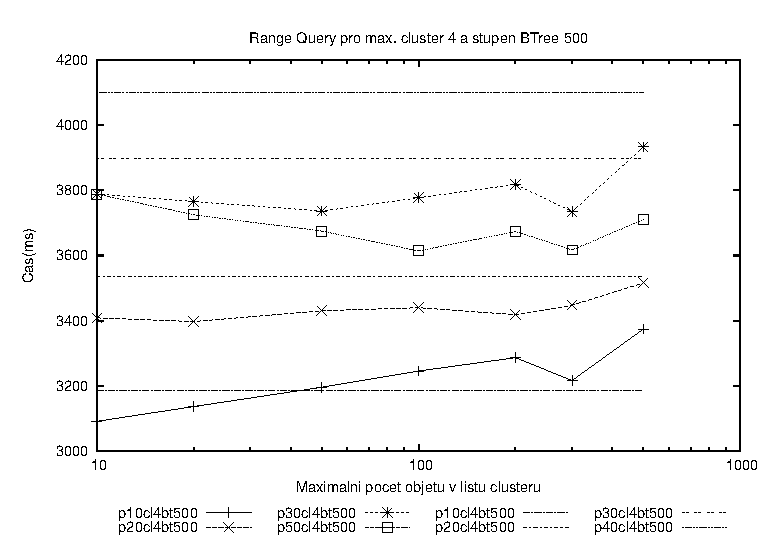
\includegraphics{jvm1_cl4_bt500}
\caption{Vliv max. počtu objektů v~listech clusteru pro JVM1}
\label{fig:jvm1cl4_bt500}
\end{figure}

\prettyref{fig:jvm1cl4_bt500} zobrazuje, jakým způsobem ovlivňuje maximální počet objektů v~listech dynamického \MIndex{u}.
Pro porovnání jsou zobrazeny i časy více-stupňového \MIndex{u}.
Ty jsou zaneseny jako vodorovné čáry.
Pro nižší počet pivotů (\num{10} a \num{20}) mají výsledné časy se zvyšujícím se počtem maximálních počtů objektů v~listech téměř lineární stoupající tendenci.
U~vyššího počtu pivotů je průběh jiný.
Není lineární a se snižujícím se max. počtem objektů v~listech (\num{10}) se dokonce zvyšuje.
Důvod, proč konfigurace s~nízkým počtem pivotů jsou dominantní je ten, že v~této konkrétní množině objektů pro vyhledávání jsou objekty shlukovány kolem konkrétních pivotů.
Utvářejí se clustery s~velkým množstvím objektů a v~jejich okolí dochází k~vyhledávání v~\BPTree{}.
Náklady při filtrování většího množství pivotů v~\emph{Range Query} jsou zřejmě signifikantní a filtrování neefektivní.

Je nutno podotknout, že při větší množině porovnávaných objektů (v~řádu stovek tisíců), by byl zřejmě \MIndex{} s~počtem pivotů 10 již nedostačující a neefektivně by rozděloval prostor.
Z~toho vyplývá, že je nutné pro každou množinu objektů odladit parametry \MIndex{u} a nelze doporučit jednu konkretní konfiguraci.

\section{Srovnání výkonu implementací v~{\protect \CC}, {\protect \CS} a Java}
Nemohl jsem použít data, které A.~Kmuníček a P.~Koman naměřili ve svých pracích\cite{Kmunicek2011thesis}\cite{Koman2012thesis}.
Srovnání výsledných časů by bylo nepřesné, protože jsem neměl k~dispozici stejné prostředí pro měření, v~kterém byly měřeny implementace v~\CC{} a \CS{}.

Po poradě s Dr.~Lokočem jsem provedl portaci původního kódu \CC{} psaného pro Windows na Linux.
Musel jsem změnit několik platformně závislých volání pro zjištění aktuálního času.
Žádné jiné změny nebyly provedeny ohledně algoritmu.
\CS{} implementace nebyla portována a nebyla tedy ani měřena.

Kolegové měřili dva dotazy o~poloměrech \num{0.15} a \num{0.25} a vyhledávaly \num{100} objektů.
Vzhledem k~tomu, že jsem pro své měření používal poloměr \num{0.15}, zvolil jsem pouze toto porovnání.
Parametry \MIndex{u} byly: vícestupňový cluster \num{3}, počet pivotů \num{10} a stupeň \BPTree{} \num{50}.

Rozhodl jsem se pro porovnání použít konfiguraci s~nejlepším časem dosaženým v~Java -- dynamický \MIndex{} s~maximálním počtem \num{10} objektů v~listu a JVM1, a také s~nejlepším výsledkem při použit stupně \BPTree{} \num{500}.

Měření probíhala s~různými parametry kompilátoru GNU\nomenclature{GNU}{GNU's Not Unix\!} \CC.
Verze kompilátoru byla (Debian 4.7.2-5) 4.7.2.

\begin{table}[h]
\center
\begin{tabular}{| l  | r | r |}
\hline
Implementace & Stupeň \BPTree & Čas (\si{\ms}) \\ \hline
\hline
\CC{} & \num{50} & \SI{2432}{\ms} \\ \hline
\CC{} (\cmd{-O3}) & \num{50} & \SI{697}{\ms} \\ \hline
\CC{} (\cmd{-O3 -march=native}) & \num{50} & \SI{408}{\ms} \\ \hline
Java JVM1 & \num{50} &  \SI{3979}{\ms} \\ \hline
Java JVM1 & \num{500} &  \SI{3500}{\ms} \\ \hline
\end{tabular}
\caption{Srovnání {\protect\CC} a Java}
\end{table}

V~tomto porovnání implementace v~\CC{} provedla \emph{Range Query} v~$\num{1.6}\times$ menším čase než Java s~parametry JVM1.
Toto je také očekávaný výsledek.
Důvodem je zřejmě \uv{masivní používání}\cite{Kmunicek2011thesis} polí a použití ukazatelové aritmetiky v~implementaci \MIndex{u} v~\CC{}.
Implementace v~Java a \CS{} využívají možnosti knihoven pro daný jazyk, např. kolekcí a zaměřily se na objektově orientovaný návrh.
Používání kolekcí umožňuje rychlejší vývoj, ale v~některých případech je toto penalizováno menší výkonností výsledného kódu.

Zajímavý je i výsledek dosažený povolením větších optimalizací -- parametry \cmd{-O3} a \cmd{-march=native} pro kompilátor.
Volba \cmd{-O3} povoluje všechny optimalizace obsažené v~\cmd{-O2}, navíc povoluje ještě tyto optimalizace: \cmd{-finline-functions}, \cmd{-funswitch-loops}, \cmd{-fpredictive-commoning}, \cmd{-fgcse-after-reload}, \cmd{-ftree-vectorize}, \cmd{-fvect-cost-model}, \cmd{-ftree-partial-pre} a \linebreak \cmd{-fipa-cp-clone}\cite{gccoptions}.
Volbou \cmd{-march=native} kompilátor používá všechny dostupné instrukce na dané architektuře.
Při kombinaci obou dvou voleb byl výsledný čas $\num{6}\times$ menší než s~výchozími volbami kompilátoru (\cmd{-O2 -g}).
Je to pravděpodobně využitím vektorových instrukcí při zpracovávání polí a v~nich uložených dat.
Nezkoumal jsem do detailů, jakým způsobem se navzájem liší kód generovaný kompilátorem \CC.

V~\prettyref{sec:memorymanagement} uvádím, že práce v~jazyce Java je bezpečnější, co se týče alokace a dealokace paměti.
Když jsem portoval implementaci \CC{}, chtěl jsem zjistit pomocí statické analýzy kódu, zda netrpí úniky paměti.
Použil jsem k~tomu volně dostupný program \cmd{cppcheck}\cite{cppcheck}.
\cmd{cppcheck} nalezl celkem \num{8} chyb při práci s~dealokováním paměti. Zde je výstup:
{\tiny
\begin{verbatim}
Checking program.cpp...
Checking program.cpp: _WIN32...
[../headers/tridy.h:72]: (error) Mismatching allocation and deallocation: BPTuzel::klice
[../headers/tridy.h:66]: (error) Mismatching allocation and deallocation: BPTuzel::data
[../headers/tridy.h:111]: (error) Mismatching allocation and deallocation: ClusterTreeNode::index
[program.cpp:614]: (error) Mismatching allocation and deallocation: poleVzdalenosti
[program.cpp:734]: (error) Mismatching allocation and deallocation: polePrvniVyberCisel
[program.cpp:678]: (error) Memory leak: polePrvniVyberCisel
[program.cpp:1464]: (error) Mismatching allocation and deallocation: polePivotu
[program.cpp:1469]: (error) Mismatching allocation and deallocation: poleVzdalenostiHledanehoBodu
Checking program.cpp: __unix__...
\end{verbatim}
}

Analýze kódu odhalila nesprávný způsob práce s~uvolňováním pole, alokovaného pomocí operátoru \method{new[]}. Místo operátoru \method{delete[]} byly uvolňovány pomocí operátoru \method{delete}\cite{Stroustrup:1997:CPL:523265}.